\question{Câu 4}

Cho mạch khuếch đại tín hiệu như hình vẽ. Giả sử các tụ có giá trị rất lớn. BJT có $\beta = 100$ và $V_{A} = \infty$.

\begin{figure}[H]
	\centering
	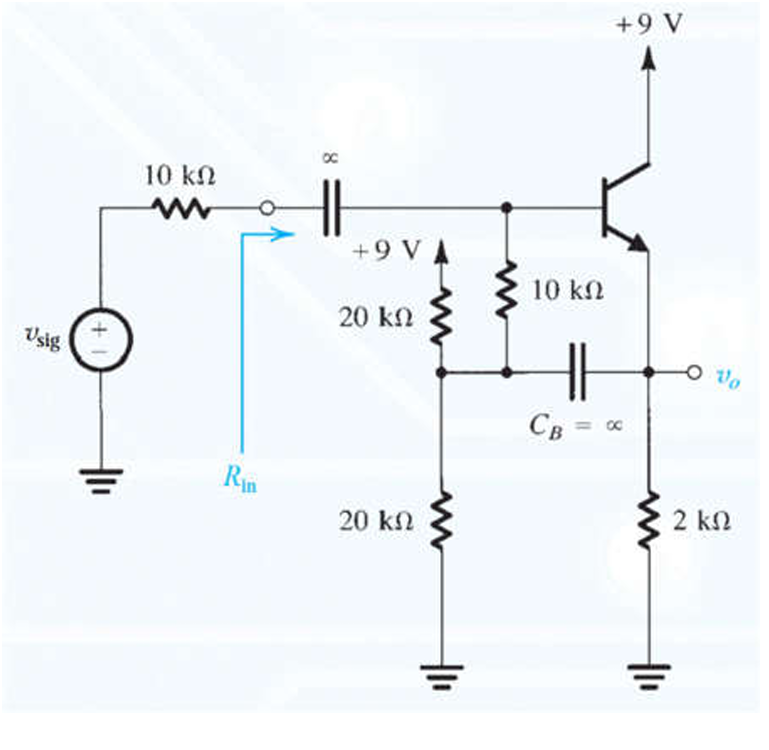
\includegraphics[width=.8\linewidth]{./my-chapters/my-images/Question4/Debai.png}
\end{figure}

\answer{a}{Tìm điểm hoạt động Q của BJT}

\noindent Xét hoạt động chế độ DC cho toàn mạch.

\begin{figure}[H]
	\centering
	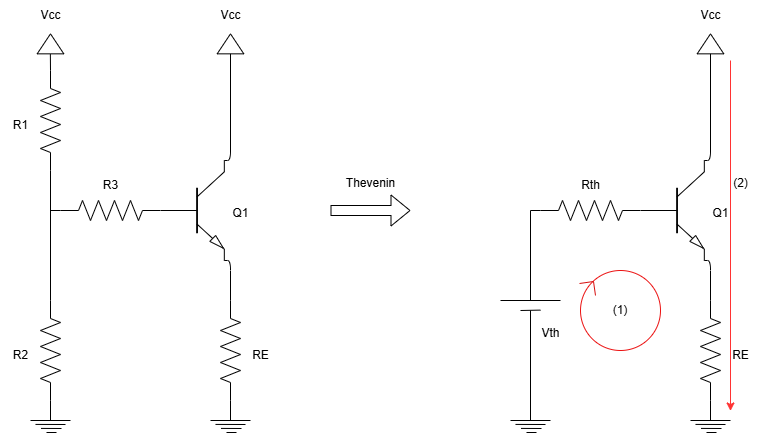
\includegraphics[width=.7\linewidth]{./my-chapters/my-diagrams/Question4/Debai.png}
\end{figure}

	Thevenin ta có:
\[ R_{th} = R_{3} + R_{1}//R_{2} = 10 + \dfrac{20\times 20}{20 + 20} = 20k\Omega\]
\[ V_{th} = \dfrac{R_{2}}{R_{1} + R_{2}} V_{cc} = \dfrac{20}{20+20} \times 9 = 4.5V\]

Áp dụng KCL cho vòng (1):
\[ -V_{th} + I_{B}R_{th} + V_{BE} + I_{E}R_{E} = 0\]
Ta có: $ I_{E} = (\beta + 1)I_{B} $
\[\Rightarrow I_{B} = \dfrac{V_{th} - V_{BE}}{R_{th} + (\beta + 1)R_{E}} = \dfrac{4.5 - 0.7}{20 + (100+1)\times 2} = 0.0171mA\]
Ta có: $I_{C} = \beta I_{B} = 100\times 0.0171mA = 1.71mA$.

Áp dụng KCL cho vòng (2):
\[ -V_{cc} + V_{CE} + I_{E}R_{E} = 0\]
Ta có: $I_{C} = \dfrac{\beta}{\beta + 1}I_{E} = \alpha I_{E} \approx I_{E}$
\[\Rightarrow V_{CE} = V_{cc} - I_{C}R_{E} = 9 - 1.71\times 2 = 5.58V \]

Vậy điểm làm việc Q của tâng 2 là : $(I_{CQ}, V_{CEQ}) = (1.710mA, 5.58V)$.

\answer{b}{Đặt $v_{s} = V_{s}\sin \left(\omega t\right)$ vào mạch. Ngõ ra nối với tải $R_{L} = 1k\Omega$. Tìm $A_{vo}$, $G_{v}$, $R_{i}$, $R_{o}$ của mạch.}

\noindent Xét hoạt động chế độ AC cho toàn mạch.

\begin{figure}[H]
	\centering
	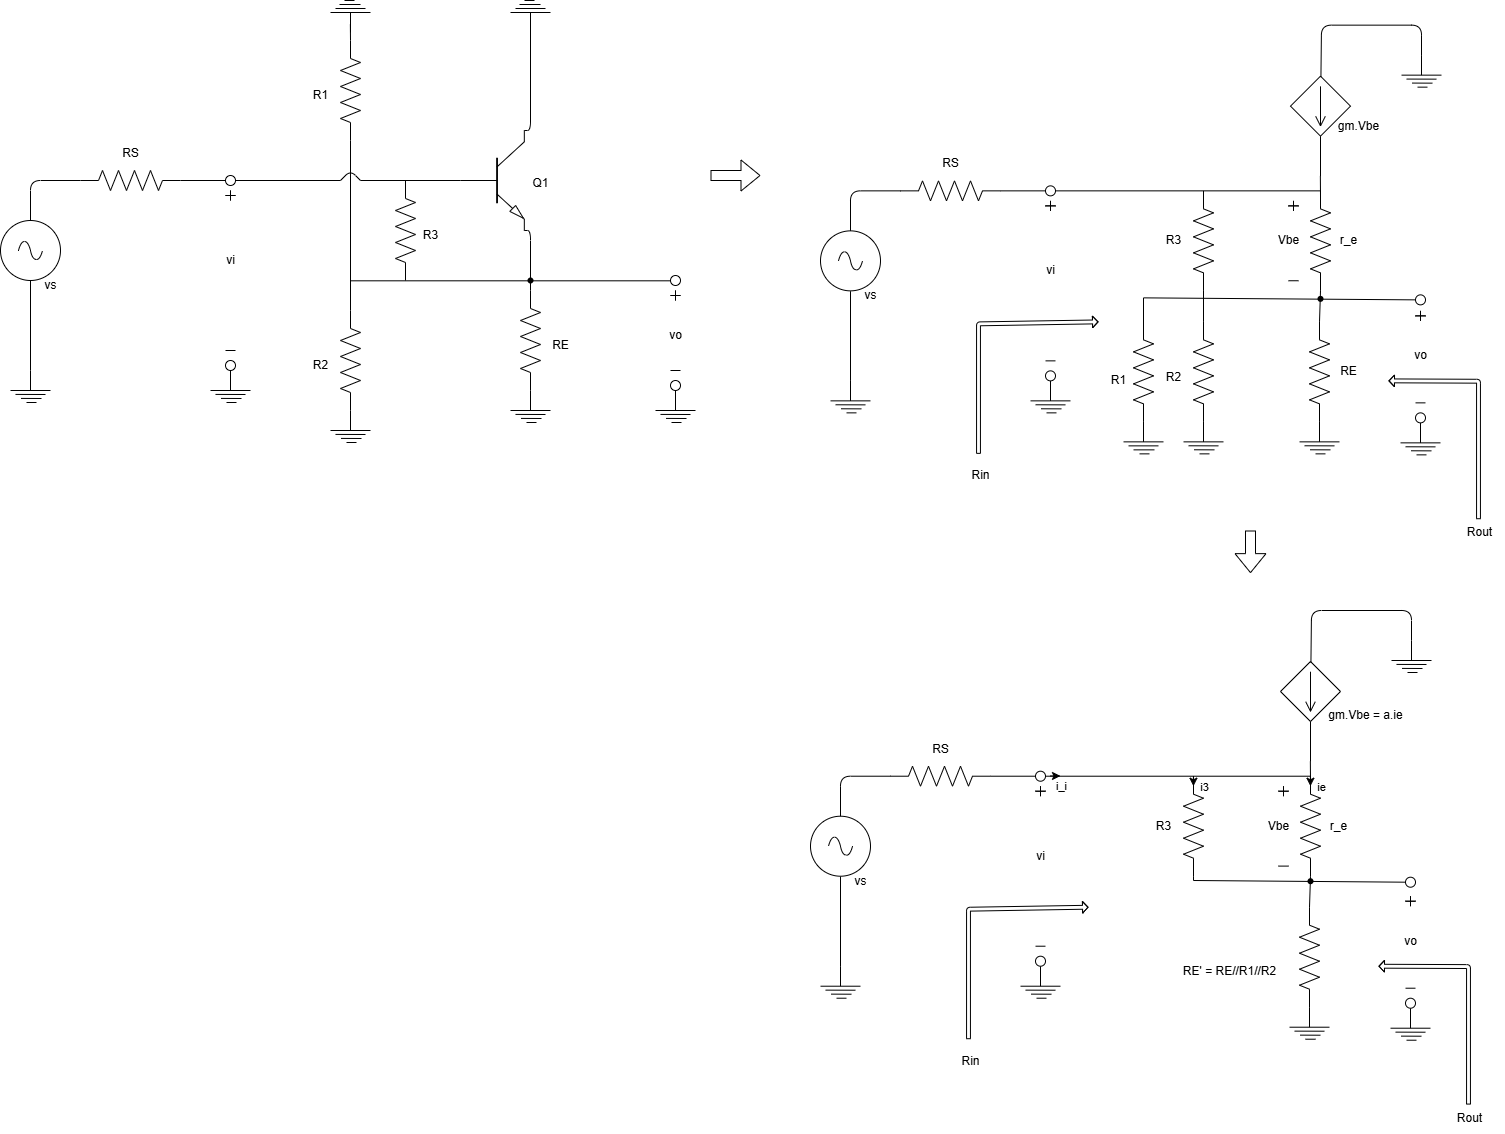
\includegraphics[width=.9\linewidth]{./my-chapters/my-diagrams/Question4/caub_t.png}
\end{figure}

\begin{itemize}[label =-]
	\item $R_{in} = \dfrac{v_{i}}{i_{i}}|_{v_{o} = 0}$
	\item $R_{out} = \dfrac{v_{o}}{i_{o}}|_{i_{i} = 0}$
	\item $A_{vo} = \dfrac{v_{o}}{v_{i}}|_{R_{L} = \infty}$
	\item $A_{v} = \dfrac{v_{o}}{v_{i}} = A_{vo}\dfrac{R_{L}}{R_{L} + R_{out}}$
	\item $G_{v} = \dfrac{v_{o}}{v_{s}} = \dfrac{R_{in}}{R_{in} + R_{s}} A_{v}$
\end{itemize}